\chapter{Desenvolvimento}
\label{cap:desenvolvimento}
Introdução do capitulo pendente 


\section{RISC-V}
\label{sec:risc-v}

As intrunçoes do conjunto RV32I são organizado dentro dos quattros formatos basicos exibidos na Figura \ref{fig:formatoInstrucaoRV32I_2}, porem para alguns cassos esses formatos puros não são suficiente para conteplar todas posibilidades, ou não são o mais eficiente, por causa disso exite algumas variçoes,  

\begin{figure}[!htb]%% Ambiente figure
     \centering % Centraliza a imagem no documento (recomendado)
     \caption{Formato das instruções da RV32I}% Legenda da sua figura
     \label{fig:formatoInstrucaoRV32I_2}%rotulo
     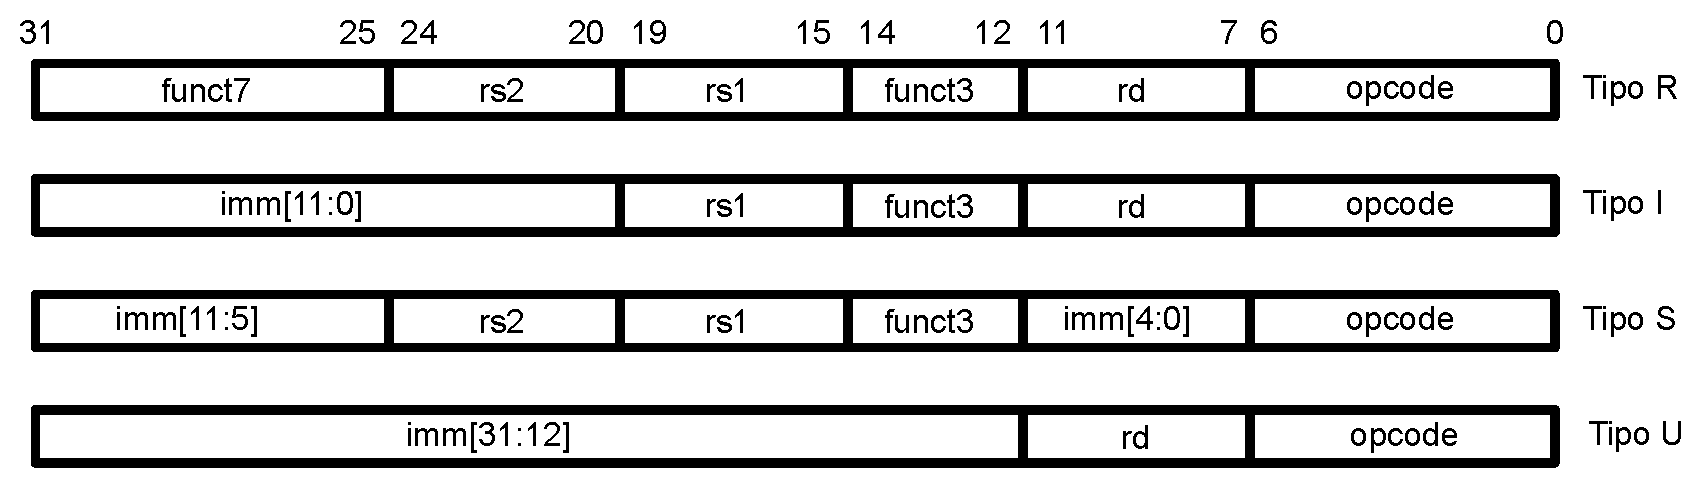
\includegraphics[scale=0.54]{figuras/instrucaoRISC-V.pdf}
     \fonte{Adaptado de \cite{riscv_manual_2026}}%% Fonte adaptada
\end{figure}

Dentro do conjunto RV32I as instruções são dividas em cinco categoraias: Inteiros, Transferência de controle, Carga e Descarga da memoria, Ordenação da memoria e Chamada de ambiente \cite{riscv_manual_2026}.

O conjunto dos inteiros é composto por 21 intruçoes e é o resposalvel por realizar as operaçoes matemticas soma e subtração, e operaçoes logicas de comapração, deslocamento, AND, OR ou XOR. A operação pode ser realizada tanto entre dois numeros vindo de registradores, quanto entre um registrador e um valor constante vindo diretemente da intrução que é nomeado de imediato.

O conjunto RV32I possui originalmente 40 instruções em sua especificação base; contudo, implementações simples como a proposta neste trabalho podem reduzir para 38 intruçoes. A primeira redução ocorre nas duas únicas instruções do tipo SYSTEM: a instrução \texttt{ECALL}, responsável por solicitar chamadas de sistema (\textit{system calls}) ao sistema operacional, e a instrução \texttt{EBREAK}, utilizada por depuradores para pausar a execução do programa e devolver o controle ao ambiente de desenvolvimento. Em um núcleo de ciclo único sem suporte a sistema operacional ou depuração em tempo real, ambas as instruções podem ser unificadas em uma rotina simplificada de exceção (\textit{trap}), disparando um sinal de interrupção ou paralisando a execução do circuito de forma controlada \cite{riscv_manual_2026}. 


Outra instrução que pode ser simplificada em implementações de escopo reduzido é a \texttt{FENCE}. Essa instrução é responsável por garantir o ordenamento na execução de memória em sistemas multicore ou em microarquiteturas avançadas com execução fora de ordem (\textit{out-of-order}). Como o processador projetado neste trabalho é de núcleo único e possui execução estritamente sequencial em ciclo único, a ordenação das operações de memória é garantida nativamente pela própria estrutura física. Dessa forma, a instrução \texttt{FENCE} torna-se redundante, podendo ser tratada funcionalmente como uma instrução NOP (do inglês \textit{No Operation}), isto é, uma operação nula que não altera o estado dos registradores nem da memória \cite{riscv_manual_2026}.


\section{Caminho de dados}
\label{sec:desenvolviemnto}

O desenvolvimento do hardware será estruturado de forma estritamente modular, dividindo a arquitetura do processador em blocos funcionais discretos e independentes, o que viabiliza a reutilização desses módulos em projetos futuros. Adota-se o modelo clássico de caminho de dados (\textit{datapath}) em ciclo único, no qual o fluxo de processamento de uma instrução ocorre integralmente dentro de um único período de \textit{clock}. A integração dessas unidades será realizada de forma hierárquica por meio de um módulo de topo (\textit{top-level}), o qual gerencia as interconexões de sinais internos, facilitando tanto as simulações comportamentais quanto a síntese física na plataforma Nexys A7.


A estrutura interna do processador será segmentada em cinco blocos principais: Unidade de Busca, composta pelo Contador de Programa (PC, do inglês \textit{Program Counter}) e por um somador dedicado; Unidade de Decodificação, constituída pelo circuito decodificador da instrução e pelo Banco de Registradores; Unidade de Execução (ALU); Unidade de Memória de dados; e Unidade de Escrita (\textit{Write-Back}). A interação simplificada entre esses blocos pode ser visualizada na Figura \ref{fig:comunicacaoBloco}. Essa partição do sistema foi projetada para garantir o isolamento de falhas durante os testes individuais e, estrategicamente, para facilitar a conversão futura da microarquitetura para o modelo segmentado em \textit{pipeline}, tomando como referência o caminho de dados estabelecido por \citeonline{hennessy2017organizacao} para um núcleo com suporte a sete instruções, \textit{ load doubleword}, \textit{store doubleword }, \textit{add}, \textit{sub}, \textit{and}, \textit{or} e \textit{beq} é ilustrado na Figura \ref{fig:caminhoDadosRiscV}.


\begin{figure}[!htb]
     \centering 
     \caption{Comunicação entre os blocos do processador}
     \label{fig:comunicacaoBloco}
     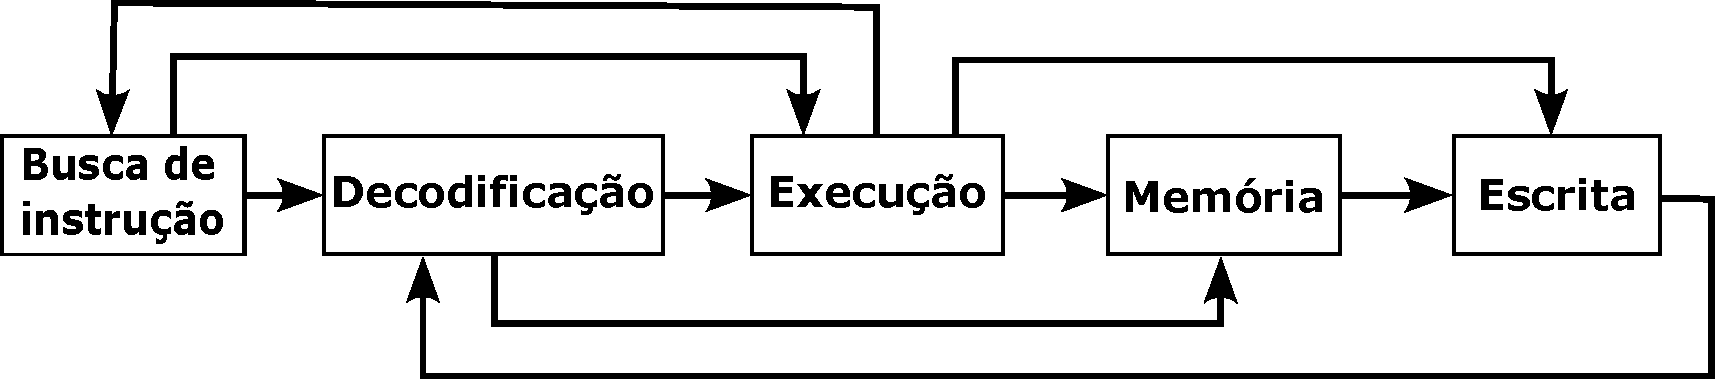
\includegraphics[scale=0.5]{figuras/FluxoProcessador.pdf}
     \fonte{Autoria própria (2026)}
     
\end{figure}

\begin{figure}[!htb]
     \centering 
     \caption{Caminho de dados de uma implementação RISC-V de ciclo único}
     \label{fig:caminhoDadosRiscV}
     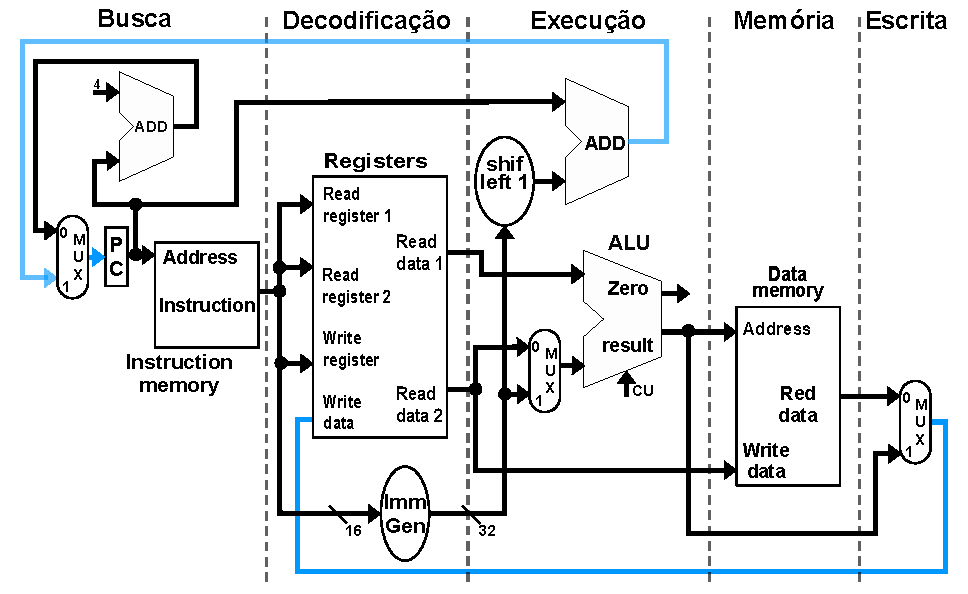
\includegraphics[scale=1]{figuras/caminhoDadosRiscV.pdf}
     \fonte{Adaptado de \citeonline{hennessy2017organizacao}}
    
\end{figure}



Para a validação de cada bloco lógico, será desenvolvido um ambiente de teste isolado (\textit{testbench}), permitindo a simulação comportamental completa do circuito e a verificação de suas funcionalidades dentro da própria suíte AMD Vivado. Cada módulo será testado individualmente e, somente após a constatação de sua estabilidade operacional, proceder-se-á com a integração hierárquica, aplicando novos estímulos de simulação a cada etapa de junção do hardware.

\subsection{ALU}


\subsubsection{Somador}

Um dos metodos mais visto para somadores na literatura é utilizando um circuito chamado de somador completo, que consite em uma pequeno circuito resposavel por realizar a soma entre dois bits de um numero, assim como realizamos a soma normalmete esse circuito soma cada digito do numero separado e se "sobrar" passa adiante essa valor para somar no proximo digito, por exemplo para realizar a soma: 

\begin{equation}
    \opadd[carrystack=true]{191}{874}
    \label{eq:soma_colunas}
\end{equation}


Em binario a podemso fazer o mesmo, e essa é a logica do soamdor compelto, soamr dois bits, e o "vai um" se existir, assim o circuito fica com 3 entradas, os dois bits a ser soamdo, o bit de vem um, conhecido com o \textit{carry-in}, e 2 saidas, o resultado da som e o bit de vai um conhecido como \textit{carry-out}, esse circuito pode ser facilemte contruido quando anlisado a tabela verdade das daus saidas

% Tabela para a Saída do Bit de Soma (S)
\begin{table}[htb]
\centering
\caption{Tabela verdade do somador completo para a saída do bit de soma ($S$).}
\label{tab:fa_soma}
\begin{tabular}{cccc}
\toprule
\textbf{A} & \textbf{B} & \textbf{$C_{in}$} & \textbf{Soma ($S$)} \\
\midrule
0 & 0 & 0 & 0 \\
0 & 0 & 1 & 1 \\
0 & 1 & 0 & 1 \\
0 & 1 & 1 & 0 \\
1 & 0 & 0 & 1 \\
1 & 0 & 1 & 0 \\
1 & 1 & 0 & 0 \\
1 & 1 & 1 & 1 \\
\bottomrule
\end{tabular}
\fonte{Elaborado pelo autor}
\end{table}

% Tabela para a Saída do Carry-Out (Cout)
\begin{table}[htb]
\centering
\caption{Tabela verdade do somador completo para o transporte de saída ($C_{out}$).}
\label{tab:fa_cout}
\begin{tabular}{cccc}
\toprule
\textbf{A} & \textbf{B} & \textbf{$C_{in}$} & \textbf{$C_{out}$} \\
\midrule
0 & 0 & 0 & 0 \\
0 & 0 & 1 & 0 \\
0 & 1 & 0 & 0 \\
0 & 1 & 1 & 1 \\
1 & 0 & 0 & 0 \\
1 & 0 & 1 & 1 \\
1 & 1 & 0 & 1 \\
1 & 1 & 1 & 1 \\
\bottomrule
\end{tabular}
\fonte{Elaborado pelo autor}
\end{table}

resultando nas equaçoes booleanas:

$$S = A \oplus B \oplus C_{in}$$
e
$$C_{out} = (A \cdot B) + (C_{in} \cdot (A \oplus B))$$

Uma subtração nada mais é que a soma entre um numero positivo e um nuemro negativo, portanto para subtarir dois nuemos basta que trasnfomemos esse nuemro em negativo utilizando a o metodo para complemteto de dois, portanto podemos utilizar uma inversora e enviar um sinal de carry-in 1

tendo as equaçoes um método de criar um soamdor seria apenas criar um somador dentro do verilog utilizando a parte logica da FPGA, porem se feito assim o caminho critico aba ficando muito grande devido a progração dos bits, para resolver isso e melhorar esse efeito de propragação de bits as FPGA possui unidade propria de alta velocidade feita para acelerar o transporte de bit chamada carry4

explciar sobre o carry4

Para utilizar os blocos carry pode ser feito utilizando operadores "+" ou "-" que ja intanciam e adicionan toda a logica nescessaria, ou intanciando eles manualmete junto da logica nescessaria. Foi realizado um teste com um progrma simples que realiza a leitura dos 16 shitchs da placa, divide ele em dois nuemos de 8 bits, send A os oito primerios bits, e B os bits mais significativo, e o resultado seria mostrado nos 16 leds, novamenet dividos em dois pares de 8 bits conforme anteriormente, para conseguir medir o tempo dos dois circuitos foi nescessario colocar um banco de registradores na entrda dos shitchs e um banco de registradores n saida dos leds.

Foi desenvolvido dois modulos, o primeiro contendo um soamdor com a feramente automatica da Listing \ref{lst:sub_auto} e o segundo da Lissting \ref{lst:sub_manula} onde alem de estanciar os dois blocos carry4 nescessario foi precisso relizar tanto a operação  de inverter o op\_b e realizar a XOR com op\_a. 


\end{lstlisting}

Obserevando os diagrmas gerado pela feramente de schematci gerado pelo virado pós-implementação é posivel observar algumas pequenas defirenças, na Figura \ref{fig:sub_auto} do circuito gerado automatico é possível observar que foi criado oito LUT e tres carry4, ja na Figura \ref{fig:sub_manual} um bloco de carry4 foi substituido por uma LUT de 1 bit.
\begin{figure}[!htb]
     \centering 
     \caption{Diagrama do circuito resultante do circuito de subtração automático}
     \label{fig:sub_auto}
     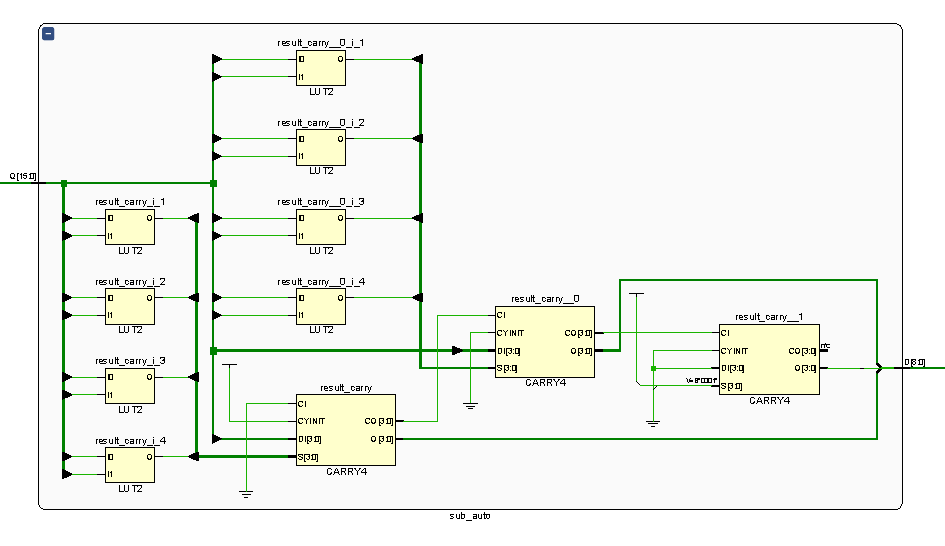
\includegraphics[scale=1]{figuras/sub_auto.pdf}
     \fonte{Autoria própria (2026)}
    
\end{figure}

\begin{figure}[!htb]
     \centering 
     \caption{Diagrama do circuito resultante do circuito de subtração manual}
     \label{fig:sub_manual}
     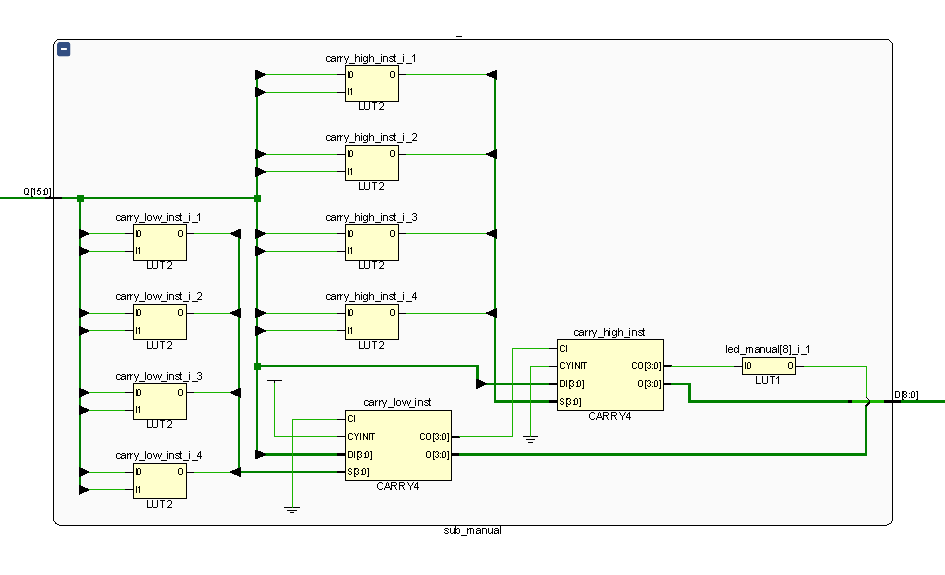
\includegraphics[scale=1]{figuras/sub_manual.pdf}
     \fonte{Autoria própria (2026)}
    
\end{figure}

Somente observar o diagrama diz nada sobre efeiciencia, para realmete conseguir definir qual o melhor é preciso fazer uma comparação entre os tempo dos caminhos criticos, para conseguir determinar a distancia entre os caminhos criticos é preciso colocar um registrador em cada entrada e saida, parra assim a feramenta de analise de timing do proprio software vivado conseguir calcular o caminho critico. Portanto foi feito o código X que intancia os registradores  e os dois modulos.


\begin{lstlisting}[language=Verilog, caption={Modulo em SystemVerilog do Subtração para comaprativo de desempenho manula}, label={lst:sub_manula}]
module top_benchmark (
    input  logic        clk,
    input  logic [15:0] switch,
    output logic [8:0]  led_auto,
    output logic [8:0]  led_manual
);
    // Registradores de Entrada
    logic [15:0] switch_reg;
    always_ff @(posedge clk) switch_reg <= switch;

    // Sinais dos submódulos
    logic [8:0] res_auto, res_manual;

    // Instanciação
    sub_auto   u_auto   (.switch(switch_reg), .clk(clk), .led(res_auto));
    sub_manual u_manual (.switch(switch_reg), .clk(clk), .led(res_manual));

    // Registradores de Saída
    always_ff @(posedge clk) begin
        led_auto   <= res_auto;
        led_manual <= res_manual;
    end
endmodule
\end{lstlisting}

Com o circuito montado é executado na ferameta de compilaççã odo código até a etapada de implemetmnação, assim permitidno utilizar a analise de design de implemtnação, dentro desse relatório o inteeresante é analise do \textit{Setup timing} dos caminhos de circuito interno, o valor desses realtorio é o tempo nescessario para que uma informação saia do registradores internos, seja processado e chege no registrador de saida, com estabilidade suficiente para garantir que o valor que será salvo é realmet o valor coreto e não algum erro causando por transição de sinal.

A Tabela \ref{tab:ComTming} contem o caminho criticos de cada circuito, é posivel tirar uma conclução finalemte, a coluna level indica a quantidade de blocos logicos que existee no caminho critico, quantos mais blocos o caminho tende a ser mais lento, e o total delay é o tempo total relamte do coircuito em nano segundos. É evidente que o caminho automatico obteve u mdesempenho  muito superior ao cominho manual, gastando aproxiamndamente 1ns a menos.

Como ficou evidente o processo onde  aferamte monta o circuito de soma automaticamente se parece ser  o mais eficiente pelo menos comaprando com uma simples 

\begin{table}[!htb]
\caption{Comparativo de timign entre o metodo de soma\label{tab:ComTming}}
    \centering
    \begin{tabular}{ccc}
         & Level & Total Delay (ns) \\
        Manual & 4 & 3,221 \\
        Atuo & 3 & 2,649 \\
    \end{tabular}
    \caption{Caption}
    \label{tab:my_label}
\end{table}



\subsubsection{Estrutura}
\label{subSub:estrutura}

Realizando um comaprativo entre a elaboração da alu, primeio o modelo mais simples onde as opçoes da ULA são definidas por um simples switch case onde cada saida é separada como no códgio X onde é implemtado uma alu de demostração. Esse modelo de implemtação é visto em diversos trbalhos, como os trabalhos de \citeonline{exem_anbalagan2026rv32i}, \citeonline{exem_hari545543_2026_rv32i}, \citeonline{exem_avelar2026granderisco5} e
\citeonline{exem_calcada2026rvx}.

Para realizar o teste foi elaborado o modulo  superior simples com registradores na entrada e saída para ser posivel utilizar a feramtena de analise de tempo.


Seguindo o mesmo padrão foi realizado um teste elaborando a ALU inpirado na implementação realizada no livro \citeonline{vahid2008sistemas}, nesse modelo é precisso dividir a ALU em dois blocos, um só responsavel pela soma, e outro chamado de extensão, querealiza qualqiuer manipulação nessecesaria. Portanto foi produzido os tres modulos, codigo x contendo sómente a intencia dos dois blocos, o código x contendo a descrição da extensão onde é realizado as modificaçoes, e por fim o codigo x soemnte realizando a soma dos valores e dando o resultado.





Alem dos dois modelos foi explorado o usso de Intenligencia Artificial generativa para tentar obter um resultado com maior velociade, par isso foi solictado as IA Gemini, ChatGpt e Claude para gerarem uma ALU similar as anterios porem do melhor meio para reduzir o tempo



A Tabela \ref{tab:alu_comparacao} foi elaborado com basse nos resultados a analise de implemtação do vivado sendo analisado o Tempo do caminho critino em ns, o consumo total e a quantidade de LUT ocupada. O consumo de energia de energia dos 5 metodos ficaram com valores praticametne iguais, de forma simila rocore nas LUT só tendo duas execoes que abaramutilizando muito mais espaço que os demais, agora o caminho critico sim ha umadifereça bem significativa  einteresante, onde o memtodo mais simples acabou tendo um tempo muito maior queo o nescessario, ja o memtodo do livro ja alcançou um resultado satisfatório, porem ainda é posivel conseguir um pouco mais de velocidade utilizando o modelo gerado pelo gemini, onde conseguiu o menor dos tempo.



\begin{table}[!htb]
  \centering
  \caption{Comparação de Métodos de Implementação de ALU em SystemVerilog no Vivado}
  \label{tab:alu_comparacao}
  \begin{tabular}{l c c c  }
    \toprule
    \textbf{Método / Origem} & \textbf{Caminho Crítico} & \textbf{Potência Total}  & \textbf{LUTs} \\
                             & (ns)                    & (W)                      &               \\
    \midrule
    Método do Livro          & 9,551                   & 0,125                   & 375            \\
    Claude                   & 9,192                   & 0,11                    & 403             \\
    Método Simples           & 7,760                   & 0,12                    & 423            \\
    GPT                      & 7,602                   & 0,111                   & 435            \\
    Gemini                   & 6,839                  & 0,111                   & 357            \\
    \bottomrule
  \end{tabular}
\end{table}


\subsubsection{Operações e I/O}
\label{subSub:operacoes}

Fazendo uma analise das intrunçoes foi determinado as operaçoes que a ULA será capaz de realizar, essas opçoes foram definidasd pensando em melhorar a velocidade das operaçoes, contemplando todas as operaçoes nscessarias confome a Tabela \ref{tab:alu_rv32i}, as operaçoes \textit{ECALL, EBREAK} e \textit{FENCE} não utilizan a ALU toda sua manipulação é relizado diretamente pela unidade de controle. 

Duas intruçoes que foram adicoandas nessa imp,emtação para reduzir ocamnho critico foram a PAS\_B evitando assi m a nescessidade de um mux para realziar a operação LUI sem qualquer interferencia do valor que tiver em A assi removendo a nescessidade de um mux apra garir valor. Outra intrução incomun é a de igualdade para assim conseguir reduzir o caminho critico evitando que todas as saidas da ALU tivesse que garantir esta zerada para sair o sinal de 1 na flag de zero, co mesta operaçã oela faz  ocomaprativo direto e colcoa no baramenteo de saida o resultado, onde o primeiro bit menso significado contem o resultado da operação, esse memso bit é o direciaonado para flag zero, apesar que ao fazer isso em outras intruçoes o valro dessa flag pode estar errado, porem como só para duas intruçoes esse dinal vai importar habilitando fica a cargo da unidade de contrle utilizar ou não. 


\begin{table}[!htb]
\centering
\caption{Mapeamento entre as Operações da ALU e as Instruções do RV32I}
\label{tab:alu_rv32i}
\begin{tabular}{lllp{5cm}}
\toprule
\textbf{Descrição / Função} & \textbf{Operação da ALU} & \textbf{Código Binário} & \textbf{Instruções RISC-V} \\
\midrule
Soma & \texttt{ADD} & \texttt{0000} & 
    \begin{tabular}[t]{@{}l@{}\texttt{ADD}, \texttt{ADDI}, \texttt{LW}, \texttt{SW}, \texttt{LB}, \texttt{LH}, \\ \texttt{LBU}, \texttt{LHU}, \texttt{SB}, \texttt{SH}, \texttt{AUIPC}\end{tabular} \\
\addlinespace
Subtração & \texttt{SUB} & \texttt{0001} & 
    \texttt{SUB}\\
\addlinespace
E Lógico & \texttt{AND} & \texttt{0010} & 
    \texttt{AND}, \texttt{ANDI} \\
\addlinespace
OU Lógico & \texttt{OR} & \texttt{0011} & 
    \texttt{OR}, \texttt{ORI} \\
\addlinespace
OU Exclusivo Lógico & \texttt{XOR} & \texttt{0100} & 
    \texttt{XOR}, \texttt{XORI} \\
\addlinespace
Deslocamento Esquerdo Lógico & \texttt{SLL} & \texttt{0101} & 
    \texttt{SLL}, \texttt{SLLI} \\
\addlinespace
Deslocamento Direito Lógico & \texttt{SRL} & \texttt{0110} & 
    \texttt{SRL}, \texttt{SRLI} \\
\addlinespace
Deslocamento Direito Aritmético & \texttt{SRA} & \texttt{0111} & 
    \texttt{SRA}, \texttt{SRAI} \\
\addlinespace
Comparação Menor Que (Com Sinal) & \texttt{SLT} & \texttt{1000} & 
    \texttt{SLT}, \texttt{SLTI}, \texttt{BLT}, \texttt{BGE} \\
\addlinespace
Comparação Menor Que (Sem Sinal) & \texttt{SLTU} & \texttt{1001} & 
    \texttt{SLTU}, \texttt{SLTIU}, \texttt{BLTU}, \texttt{BGEU} \\
 \addlinespace
Comparação de igualdade&\texttt{CMP}& \texttt{1011}&\texttt{BEQ}, \texttt{BNE}\\
\addlinespace
Passagem Direta do Operando B & \texttt{PASS\_B} & \texttt{1010} & 
    \texttt{LUI},  \texttt{JAL}, \texttt{JALR} \\

\bottomrule

\end{tabular}
\end{table}


Para este projeto as entradas composta por dois baramenteos de dados  A e B com 32 bits e um baramento de seleção com quatros bits. A saida será composta por um barramento de 32 bits com os dados, e um bit indicando se o resultado da ALU é zerro, se dá a nescessidade desse bit zerro para as intruçoes de desvio \textit{BEQ} e \textit{BNE} onde é precisso realizar uma comparação para ver se os valores são iguais, para isso realiza uma subtração e verifica se o valor é zero, onde só será zero se os dosi valores de entrada forem ezatamente igual, até mesmo o sinal. 

\subsubsection{Validação ALU}
\label{subSub:tb_alu}

para validar a alu finalizada e garatir sua integridade é preciso pasala por um testbench, nesse testbench autmatico é ingetado valores na ula conehcido e comparado com esperados, alem de gerar mil valores aleatório para que memos com varios continua valido os resultados, para isso utilizace uma função dentro do ambiente de simulaçao que tambme recebe as entrada s epoduz uma saida. Ao final o sistema monta u mrelatório infomando se algu mvalor não corepondeu coretamente ao esperado.

inserido onze teste de forma manual  e mil automaticos, todos pasaram com sucesso, valdiando assim o funcionamento da alu.



\subsection{BUSCA}
\label{sub:busca}

Uma intrução de 32 bits é dividida em 4 bytes, onde cada uma fica seguido após a outra como uma pilha de intrução, o é um simples registrador de 32 bits que armazena o endereço que aintrução atual esta dentro da memoria de intrução.

image

o modulo de busca de intrução é relativamente simplples, compsoto por um registrador de progrma (PC, do ingles \textit{Progrman count}), esse registrador guarda o valor da intrução que será 

O tamanho da memoria de intruçoes pode chegar até (valor maximo), porem para esta aplicação não é nescessario tão grande portanto será utilizado apenas 1024 endereços.

para o modulo de busca ficou com cinco entradas e tres saidas. Uma entrada para   o \textit{clock} (clk), uma para reiniciar o modulo (rest_i), uma para permitir a escrita no registrador pc (pq_write_i), essas entradas não serão utilzadas normalmente, são apenas para iniciação e controle manual, um baramento com novo endereço do desvio (new_pc_i) e um bit de controle para realizar o desvio para o endereço do new_pc_i (pc_branch_i), essas etradas é para realizar todas as intruçoes de desvio coretamente.

As saidas serão composta pela intrção que foi lida da memoria (instr_o), o atual valor do pc, que será utilizado para o calcular do endereço de desvio (pc_o) e o valor de pc mais quatro, que representa  oproximo endereço casso não acontença nenhum desvio, esse valor será armazenados nas intruçoes JAL e JAR

O modulo possui funcionanmenteo simples, a cada mudança de clock ele atualiza o valor do contandor do pc, ou para o valor pc + 4 ou para o endereço do desvio. O valor do pc é diividido em tres caminhos, para ler o valro da INTRUÇÃO, soamr 4 ou para saida.

PAra realizar a valição do blocoo foi elaborado um testbanch, onde faço ele ter um comportamento conehcido, que posso prever o resultado e inserir o valor esperado, assim o modulo ja compara o valor do resultado com o valor informado como esperado, como o modulo atualiza seu valor na borda de subida do clock, todas as atualizaçoes no ambiente de simulação devem ocrer no meio, para que assim todos os sinasi que precisarem consigam se propragar coretamente, para isso pode ser utilizado no teste a borda de descida do clock para atualizar os valores e verifica se a alteração que ocoreu na operaçao anterior está coreta.

Todos os teste pasaram perfeitamente nessa estapa.

\subsection{Execução}
\label{sub:executar}

A unidade de Execução é compsota por duas partes, a ALU e bloco de desvio.

Para comteplar todas as intruções do conjuunto rv32i é preciso que as entradas da ALU alterem dependnendo da intrução, na entrada A para a maioria das intruçoes entra o valor do registrador um, porem para a intrução AUIPC é preciso ter o valor do pc, portanto na entrada A entrar´o pc ou imm, sendo definidio pelo sinal de controle control_alu_a vindo da CU.

A entrda B da ALU, ja pode assumir tres valores, o valrodireto do resgistrador 2 para intruçoes do tipo R e tipo B, para as intruçoes de desvio incondicional será posivel etrarr o valor de pc + 4, para assim registrar ela nos registradores, essa escolha foi tomada com o bjetivco de reduzir o caminho critico evitando um mux na entrada da memoria do registrador, para as demais intruçoes o valor sera o imm deslocado um bit para esquerda, esse deslocamneto é definido pela propria rv322i para garantir o alinhamento da memoria.

a segunda parte do bloco de execução é o gerador de endereço de desvio, esse bolco conta cum um somador proprio, como todas as operaçoes de desvios foram colocadas para esse somador é preciso colocar um mux em uma de sus entradas, de todas as intruçoes de desvio, condicionais ou incondicionais, só uma realiza uma operação diferente de pc + imm, que seria  intrução jalr onde faz rs1 + imm, portanto sóemnte quando for essa intrução um das entradas do somador deve ser trocada para o valor de pc para o registrador 1. 


alem de determinar o endereço para qual sera desviado, esse bloco tambem ´utilizado para determinar se deve ou não realizar o desvio, princiapalmete para os desvios incondicionais, onde esse bloco utiliza o valor da saida zerro da ULA junto com sisnais de controle do CU, para determinar em cada uma das quatro situaçoes, (salto condiconal condição verdaderria, salto coniconal condição falsa, salto incondicioanl relativo ao pc, salto incondicional relativo ao rs1) se deve saltar ou não.



para validar o funcionamento foi realizado um testbench contendo 34 teste, testando todas as operaçoes da ALU, com as diferentes entradas possiveis, e testado os 4 diferentes saltos posiveis, os teste foam ralizados de forma automatica e todos passaram na validação.

\subsection{Memoria de dados}
\label{sub:memoeria_dados}

O módulo de memória de dados (\texttt{data\_memory}) possui uma entrada para o sinal de relógio (\texttt{clk}), uma entrada para habilitar a escrita (\texttt{mem\_write\_i}), um sinal para a largura do acesso (\texttt{mem\_width\_i}, especificando byte de 8 bits, meia-palavra de 16 bits ou palavra de 32 bits), um indicador de extensão de sinal para o valor lido (\texttt{mem\_signed\_i}), além de um barramento para o endereço de byte da leitura ou escrita (\texttt{addr\_i}), um barramento com o dado a ser gravado na memória (\texttt{data\_i}) e por fim 4 barramentos de 32 bits para mapeamento de entrada  (\texttt{io\_in0\_i} a \texttt{io\_in3\_i}).


O módulo fornece uma única saída para o \textit{datapath}, \texttt{data\_o}, contendo o valor lido devidamente alinhado e estendido para 32~bits. Adicionalmente, quatro saída de 32 bits mapeada em memória (\texttt{io_out0\_o} a \texttt{io\_out3\_o}).

O conteúdo inicial da memória é carregado a partir do arquivo especificado pelo parâmetro \texttt{MEM\_FILE} (cujo valor padrão é \texttt{data.mem}), através da diretiva \texttt{\$readmemh}. Esse arquivo armazena um byte por posição em ordem crescente de endereço, sendo gerado pelo fluxo de compilação a partir das seções de dados do programa (\texttt{.data} e \texttt{.rodata}). A inicialização ocorre exclusivamente durante a configuração do FPGA; o sinal de \textit{reset} do processador reinicia apenas o registrador \textit{Program Counter} (PC), mantendo o conteúdo da memória inalterado.

\subsection{Armazenamento}

A memória é composta por 1024 palavras de 32~bits, totalizando 4~KiB (definida pelo parâmetro \texttt{MEM\_DEPTH}). Cada palavra agrupa quatro bytes na ordenação \textit{little-endian}, conforme a especificação da arquitetura RISC-V. 

Por tratar-se de um processador monociclo, a leitura deve ocorrer de forma combinacional, disponibilizando o dado no mesmo ciclo de clock em que o endereço é calculado. Uma vez que os blocos de memória dedicada (BRAM) do FPGA operam com leitura síncrona (apresentando latência de um ciclo), optou-se pela implementação da memória em RAM distribuída (LUTRAM), construída a partir das tabelas de busca (LUTs) do dispositivo. 

A memória foi descrita como uma matriz bidimensional de bytes, contendo em cada espaço de endereçamento 1 byte (8bits) e em cada linha 4 espaços, assim cada endereço representa 32 bits dividido em 4 partes, a quantidade padrão de endereços gerados é de 1024.

\subsubsection{Operação de Leitura e Escrita}
\label{subsub:escritaLeitura}

Na leitura, a palavra endereçada é recuperada integralmente. Para acessos em nível de byte, ou meia-palavra, a posição selecionada pelos bits \texttt{addr[1:0]} é direcionada aos 8~bits menos significativos. Os bits remanescentes passam por extensão de sinal (instruções \texttt{LB} e \texttt{LH}) ou por preenchimento com zeros (\texttt{LBU} e \texttt{LHU}).

 A escrita só ocorre na borda de subida do sinal de clock quando \texttt{mem\_write\_i} está em nível alto (1). Alem de permitir escolher se deseja escrever em só um byte, meia-palavra ou palavra inteira de acordo com o sinal de controle \texttt{mem\_width\_i}:
\begin{itemize}
    \item \texttt{SB}: habilita apenas o byte endereçado;
    \item \texttt{SH}: habilita os dois bytes pertencentes à meia-palavra endereçada;
    \item \texttt{SW}: habilita os quatro bytes simultaneamente.
\end{itemize}

quando uma operação de escrita vai ser realizada em byte ou meia palavra o dado de entrada é replicado em toda palavra. Dessa forma, em uma operação \texttt{SB}, o byte de dado é replicado em todas as quatro posições, garantindo que a faixa habilitada receba o valor correto. 

Acessos de meia-palavra e palavra exigem alinhamento de endereço; acessos desalinhados não são suportados e não geram exceções de hardware.

\subsubsection{Mapa de Endereçamento}
\label{subsub:enderecamento}

O espaço de endereçamento da memória é estruturado conforme a seguir:
\begin{itemize}
    \item \texttt{0x0000\_0000} a \texttt{0x0000\_0FFF}: Memória RAM principal;
    \item \texttt{addr[31:28] = 4} (endereço base \texttt{0x4000\_0000}): Espaço reservado para E/S (MMIO);
    \item Endereços fora desses intervalos: a leitura retorna zero e as operações de escrita são ignoradas.
    
\end{itemize}

No espaço de E/S, as quatro portas de saída ocupam os endereços de \texttt{0x4000\_0000} a \texttt{0x4000\_000C}. Tratam-se de registradores de 32~bits com suporte a escrita parcial por byte (seguindo a mesma lógica da RAM) e não permite leitura. As quatro portas de entrada ocupam os endereços \texttt{0x4000\_0010} a \texttt{0x4000\_001C} e operam exclusivamente em modo de leitura. A seleção de largura e a extensão de sinal nas portas de E/S seguem as mesmas regras aplicadas à RAM. 

As portas possuem interface genérica, cabendo ao módulo de topo o mapeamento para os periféricos.
Essa abstração garante que o núcleo do processador permaneça independente das especificidades do hardware periférico.

\subsubsection{Verificação e Testes}
\label{subsub:testebenchMemoriaDados}

A validação foi conduzida por meio do \textit{testbench} automatizado \texttt{tb\_data\_memory}, que aplica os estímulos na borda de descida do clock e verifica as respostas imediatamente após a borda de subida subsequente. Em cada caso de teste, o sinal de saída \texttt{data\_o} é comparado com o valor esperado, e os quatro bytes da palavra são inspecionados diretamente na estrutura da memória, assegurando a seletividade das escritas parciais.

O plano de testes cobriu:
\begin{itemize}
    \item Leitura e escrita de palavras, meias-palavras e bytes (com e sem extensão de sinal);
    \item Reconstituição de uma palavra de 32~bits a partir de quatro escritas consecutivas em nível de byte;
    \item Validação de inibição de escrita com \texttt{mem\_write\_i} em nível baixo (0);
    \item Acesso aos limites da memória (última posição).
\end{itemize}

Na verificação do subsistema de E/S, avaliou-se:
\begin{itemize}
    \item Escrita e leitura das quatro portas de saída;
    \item Operação de escrita parcial por byte nos registradores de saída;
    \item Leitura das quatro portas de entrada com extensão de sinal;
    \item Rejeição de escrita em portas de entrada ou em endereços não mapeados;
    \item Isolação entre operações de E/S e a memória RAM.
\end{itemize}

A suíte completa de 46 testes obteve 100\% de aprovação.

\subsection{Escrita}
\label{sub:escrita}

O bloco de escita no registradores é o bloco responsavel por escolher qual dado deve ser salvo nos registradores se é um valor vindo da memoria ou um valor vindo do ALU, portato ese modulo só precisa das entrdasm o valor vindo da memoria (mem_data_i), a entrada vindo da saida da ALU (alu_result_i) e uma entrada de controle vindo do bloco de controle (mem_to_reg_i), e para saidas bastauma saida com a escolha do resutlado (wb_data_o).

Quando o valor da entrada mem_to_reg_i estiver 0 a saida sera ovalor do resultado da alu, e quanfo for 1 saira o valro mem_to_reg_i. 

Algumas implemtnaçoe  observadas, como a do \citeonline{exem_hari545543_2026_rv32i}e do \citeonline{exem_calcada2026rvx} utilizan nessa etapa tambem para entrada do valor com contador de programa mais quatro, porem com ofoi adiconado direto na entrada do bloco de execução com o bejtivo de otimizar os seletores não será preciso aqui.

Para validação desse bloco foi elaborado um testebench simple automatizado aplicando mudnaa do valor na borda de decida e ja verificando o resultado. todos teste passaram.

\subsection{Decodificação}
\label{sub:decodificacao}


\subsubsection{Registrador}
\label{subsub:registrador}

Para o modulo de registro ficoiu com uma entrada para \textit{clock} (clk), uma entrada parahabilitar a escrita (written_enable_i), um baramenteo de 32 bits com os dados a serem escritos (written_data_i), um abarementeo com 5 bits por padrão com o endereço de escrita (written_add_i), outros dois baramento de 5 bits co mendereço do registro que ddeve ser lido no rs1 e rs2 (rs1_add_i e rs2_add_i) e apra saida doi baramento de 32 bits com os dados lidos (rs1_o e rs2_o).

Este modulo foi elaborado de form asimpels utilziando a declaração de como array de 31 posiçoes (1:31) ja que o registradr 0 por definição da RV31I deve ser semore 0 sendo imposivel de escrever nele, assim com o bjetivo de simplificar foi gerado apenas 31 valores.

Tanto para escrita quandot leitura foi adicionado um verificador de condição para garantir que quando o endereço seja 0 de 0 na saida e não faça nada na entrada, apesar de adiianr um bloco de logica mais alem da propria seleção antural da estrutura de array após compilação do código o resultado é otimizado e esse bloco desaparece se tornand parte do conjunto compelto de registradores.

Para fim de garatir foi realizado um pequeno testbench automatico que valida se os dados estão sendo salvos coretamente no registrador e as leituras então coretas, todas a lteraçoes de siansi raealizadas na bordsa de descida e todas as verificaçoes na borda de subiida, ja que este é um compoennte sincrino de borda de subida. 

\subsubsection{Gerado de Imaediato}
\label{subsub:imm_gen}


O gerador de imediato é o bloco capaz de pegar um valor que está no meio da intrução e deixalo formato e com tamanho coreto para execução para o resto do circuito. Para esse gerador é preciso somente entrda da intrução completa com 32 bits (instruction_i), e a saida com 32 bits do valor pronto (imm_o).

O formato da decodificaçã ode uma intrução varia confome o tipo e variação de ada uma, e para identificar o tipo basta a nalisar o opconde da intrução (7 priemrios bits) e assim codificar ela para o capçar confome especificado pela isa rv32i.

Foi realizado um testbench automatico para este modulo onde os dados são inseridos na borda de escida e ja verificado a resposta, todos os teste passaram coretamente.

\subsubsection{Control unit}
\label{subsub:control_unit}

A unidade de controle (\textit{control unit}) recebe a instrução completa de 32 bits por meio da entrada \texttt{instruction\_i}. A partir dos campos \textit{opcode}, \textit{func3} e \textit{func7}, o bloco identifica a operação e gera os sinais usados pelas etapas de execução, acesso à memória, escrita no banco de registradores e atualização do contador de programa. A unidade é combinacional e não possui entrada de clock.


As portas da unidade e sua relação com os blocos do processador estão descritas na Tabela~\ref{tab:control-unit-ports}. Os prefixos dos nomes das saídas indicam o módulo que recebe cada sinal. Os sinais de largura e extensão de memória usam os tipos definidos em \texttt{mem\_pkg}; os sinais da ALU e dos desvios usam os tipos definidos em \texttt{alu\_pkg} e \texttt{branch\_pkg}.

\begin{table}[!htb]
\centering
\caption{Entradas e saídas da unidade de controle.}
\label{tab:control-unit-ports}
\begin{tabular}{p{4.1cm}p{2.1cm}p{8.0cm}}
\toprule
\textbf{Sinal} & \textbf{Direção / largura} & \textbf{Descrição} \\
\midrule
\texttt{instruction\_i} & Entrada, 32 bits & Instrução completa a ser decodificada. \\
\texttt{execution\_alu\_control\_o} & Saída, \texttt{alu\_op\_t} & Seleciona a operação da ALU. \\
\texttt{execution\_branch\_control\_o} & Saída, \texttt{branch\_op\_t} & Seleciona a condição ou a origem do desvio. \\
\texttt{execution\_branch\_enable\_o} & Saída, 1 bit & Habilita a avaliação de desvio em \texttt{execution}. \\
\texttt{execution\_control\_alu\_a\_o} & Saída, 1 bit & Seleciona rs1 (0) ou PC (1) para a entrada A da ALU. \\
\texttt{execution\_control\_alu\_b\_o} & Saída, 2 bits & Seleciona rs2 (\texttt{00}), imediato (\texttt{01}) ou PC+4 (\texttt{10}) para a entrada B da ALU. \\
\texttt{search\_pc\_write\_o} & Saída, 1 bit & Habilita a atualização do PC; nesta implementação permanece em 1. \\
\texttt{data\_memory\_mem\_write\_o} & Saída, 1 bit & Habilita a escrita na memória de dados. \\
\texttt{data\_memory\_mem\_width\_o} & Saída, \texttt{mem\_width\_t} & Define acesso a byte, meia palavra ou palavra. \\
\texttt{data\_memory\_mem\_signed\_o} & Saída, \texttt{mem\_signed\_t} & Define extensão com ou sem sinal durante loads. \\
\texttt{register\_file\_written\_enable\_o} & Saída, 1 bit & Habilita a escrita do resultado no registrador destino. \\
\texttt{write\_back\_mem\_to\_reg\_o} & Saída, 1 bit & Seleciona dado da memória (1) ou resultado da ALU (0) no write-back. \\
\bottomrule
\end{tabular}
\end{table}

Por padrão, a unidade seleciona \texttt{OP\_ADD}, mantém os desvios desabilitados, não escreve na memória nem no banco de registradores e seleciona o resultado da ALU para write-back. O seletor de largura de memória assume \texttt{MEM\_WIDTH\_WORD}, e o seletor de extensão assume \texttt{MEM\_UNSIGNED}. O sinal \texttt{search\_pc\_write\_o} permanece ativo. Esses valores também são mantidos para opcodes não suportados.

Nas tabelas de decodificação, os campos \textit{opcode}, \textit{func3} e \textit{func7} mostram a codificação da instrução RV32I. Um traço (--) indica que o campo não é aplicável àquele formato ou não participa da seleção descrita. Salvo quando indicado, as saídas não mencionadas em cada classe mantêm os valores padrão apresentados acima.

\paragraph{Operações da ALU.}
A Tabela~\ref{tab:control-unit-alu-decode} resume as instruções aritméticas, lógicas e de deslocamento. Em todas elas, a escrita no registrador destino é habilitada. Para instruções do tipo R, a entrada A recebe rs1 e a entrada B recebe rs2. Para instruções do tipo I, A recebe rs1 e B recebe o imediato. O campo \textit{func7} só diferencia as operações indicadas na tabela; para as demais operações, a implementação não usa esse campo na seleção da ALU.

\begin{table}[!htb]
\centering
\caption{Decodificação das instruções que utilizam a ALU.}
\label{tab:control-unit-alu-decode}
\begin{tabular}{lllll}
\toprule
\textbf{Instrução} & \textbf{opcode} & \textbf{func3} & \textbf{func7} & \textbf{Operação da ALU} \\
\midrule
ADD   & \texttt{0110011} & \texttt{000} & \texttt{0000000} & \texttt{OP\_ADD} \\
SUB   & \texttt{0110011} & \texttt{000} & \texttt{0100000} & \texttt{OP\_SUB} \\
SLL   & \texttt{0110011} & \texttt{001} & \texttt{0000000} & \texttt{OP\_SLL} \\
SLT   & \texttt{0110011} & \texttt{010} & \texttt{0000000} & \texttt{OP\_SLT} \\
SLTU  & \texttt{0110011} & \texttt{011} & \texttt{0000000} & \texttt{OP\_SLTU} \\
XOR   & \texttt{0110011} & \texttt{100} & \texttt{0000000} & \texttt{OP\_XOR} \\
SRL   & \texttt{0110011} & \texttt{101} & \texttt{0000000} & \texttt{OP\_SRL} \\
SRA   & \texttt{0110011} & \texttt{101} & \texttt{0100000} & \texttt{OP\_SRA} \\
OR    & \texttt{0110011} & \texttt{110} & \texttt{0000000} & \texttt{OP\_OR} \\
AND   & \texttt{0110011} & \texttt{111} & \texttt{0000000} & \texttt{OP\_AND} \\
\addlinespace
ADDI  & \texttt{0010011} & \texttt{000} & -- & \texttt{OP\_ADD} \\
SLTI  & \texttt{0010011} & \texttt{010} & -- & \texttt{OP\_SLT} \\
SLTIU & \texttt{0010011} & \texttt{011} & -- & \texttt{OP\_SLTU} \\
XORI  & \texttt{0010011} & \texttt{100} & -- & \texttt{OP\_XOR} \\
ORI   & \texttt{0010011} & \texttt{110} & -- & \texttt{OP\_OR} \\
ANDI  & \texttt{0010011} & \texttt{111} & -- & \texttt{OP\_AND} \\
SLLI  & \texttt{0010011} & \texttt{001} & \texttt{0000000} & \texttt{OP\_SLL} \\
SRLI  & \texttt{0010011} & \texttt{101} & \texttt{0000000} & \texttt{OP\_SRL} \\
SRAI  & \texttt{0010011} & \texttt{101} & \texttt{0100000} & \texttt{OP\_SRA} \\
\bottomrule
\end{tabular}
\end{table}

Nas linhas em que \textit{func7} aparece como --, esse campo não é verificado pela unidade para selecionar a operação. Em SLLI e nos deslocamentos à direita imediatos, os bits superiores do imediato ocupam a posição correspondente a \textit{func7}; a unidade compara esses bits com os padrões de deslocamento definidos em \texttt{func7\_pkg}.

\paragraph{Acessos à memória.}
Para loads e stores, a ALU soma rs1 ao imediato, com \texttt{execution\_control\_alu\_b\_o = 01}. A Tabela~\ref{tab:control-unit-memory-decode} apresenta os campos e sinais específicos de cada operação.

\begin{table}[!htb]
\centering
\small
\caption{Decodificação das instruções de acesso à memória.}
\label{tab:control-unit-memory-decode}
\begin{tabular}{llllllll}
\toprule
\textbf{Instrução} & \textbf{opcode} & \textbf{func3} & \textbf{func7} & \textbf{ALU} & \textbf{Largura} & \textbf{Sinal} & \textbf{Controles ativos} \\
\midrule
LB  & \texttt{0000011} & \texttt{000} & -- & \texttt{OP\_ADD} & Byte & Com sinal & RegWrite, MemToReg \\
LH  & \texttt{0000011} & \texttt{001} & -- & \texttt{OP\_ADD} & Half & Com sinal & RegWrite, MemToReg \\
LW  & \texttt{0000011} & \texttt{010} & -- & \texttt{OP\_ADD} & Word & Com sinal & RegWrite, MemToReg \\
LBU & \texttt{0000011} & \texttt{100} & -- & \texttt{OP\_ADD} & Byte & Sem sinal & RegWrite, MemToReg \\
LHU & \texttt{0000011} & \texttt{101} & -- & \texttt{OP\_ADD} & Half & Sem sinal & RegWrite, MemToReg \\
\addlinespace
SB  & \texttt{0100011} & \texttt{000} & -- & \texttt{OP\_ADD} & Byte & -- & MemWrite \\
SH  & \texttt{0100011} & \texttt{001} & -- & \texttt{OP\_ADD} & Half & -- & MemWrite \\
SW  & \texttt{0100011} & \texttt{010} & -- & \texttt{OP\_ADD} & Word & -- & MemWrite \\
\bottomrule
\end{tabular}
\end{table}

Nas linhas de load, \texttt{RegWrite} corresponde a \texttt{register\_file\_written\_enable\_o} e \texttt{MemToReg} a \texttt{write\_back\_mem\_to\_reg\_o}. Para stores, \texttt{MemWrite} corresponde a \texttt{data\_memory\_mem\_write\_o}; a escrita no banco de registradores permanece desabilitada. O campo \textit{func7} não é usado para decodificar loads ou stores.

\paragraph{Desvios condicionais.}
Todos os desvios usam rs1 e rs2 nas entradas da ALU e mantêm a escrita em registrador e memória desabilitada. A Tabela~\ref{tab:control-unit-branch-decode} apresenta a seleção da comparação e da condição de desvio.

\begin{table}[!htb]
\centering
\caption{Decodificação dos desvios condicionais.}
\label{tab:control-unit-branch-decode}
\begin{tabular}{llllll}
\toprule
\textbf{Instrução} & \textbf{opcode} & \textbf{func3} & \textbf{func7} & \textbf{ALU} & \textbf{branch control} \\
\midrule
BEQ  & \texttt{1100011} & \texttt{000} & -- & \texttt{OP\_CMP}  & \texttt{OP\_BCT} \\
BNE  & \texttt{1100011} & \texttt{001} & -- & \texttt{OP\_CMP}  & \texttt{OP\_BCF} \\
BLT  & \texttt{1100011} & \texttt{100} & -- & \texttt{OP\_SLT}  & \texttt{OP\_BCT} \\
BGE  & \texttt{1100011} & \texttt{101} & -- & \texttt{OP\_SLT}  & \texttt{OP\_BCF} \\
BLTU & \texttt{1100011} & \texttt{110} & -- & \texttt{OP\_SLTU} & \texttt{OP\_BCT} \\
BGEU & \texttt{1100011} & \texttt{111} & -- & \texttt{OP\_SLTU} & \texttt{OP\_BCF} \\
\bottomrule
\end{tabular}
\end{table}

Para as seis instruções, \texttt{execution\_branch\_enable\_o = 1}. A implementação da etapa de execução interpreta \texttt{OP\_BCT} como aceitar quando o bit de condição da ALU é 1 e \texttt{OP\_BCF} como aceitar quando esse bit é 0. No projeto, a saída chamada \texttt{zero\_o} da ALU acompanha o bit menos significativo do resultado; assim, \texttt{OP\_CMP} fornece o resultado da comparação de igualdade e \texttt{OP\_SLT}/\texttt{OP\_SLTU} fornecem os resultados das comparações relacionais.

\paragraph{Saltos e instruções de imediato superior.}
A Tabela~\ref{tab:control-unit-jump-upper-decode} reúne as instruções que selecionam o PC ou o imediato superior. Para JAL e JALR, o resultado de write-back é PC+4, enquanto o destino do salto é calculado na etapa de execução.

\begin{table}[!htb]
\centering
\small
\caption{Decodificação de saltos e instruções do tipo U.}
\label{tab:control-unit-jump-upper-decode}
\begin{tabular}{llllllll}
\toprule
\textbf{Instrução} & \textbf{opcode} & \textbf{func3} & \textbf{func7} & \textbf{ALU} & \textbf{A / B} & \textbf{Desvio} & \textbf{RegWrite} \\
\midrule
LUI   & \texttt{0110111} & -- & -- & \texttt{OP\_PASS\_B} & -- / imediato & Desabilitado & 1 \\
AUIPC & \texttt{0010111} & -- & -- & \texttt{OP\_ADD}    & PC / imediato & Desabilitado & 1 \\
JAL   & \texttt{1101111} & -- & -- & \texttt{OP\_PASS\_B} & -- / PC+4 & \texttt{OP\_BIP} (1) & 1 \\
JALR  & \texttt{1100111} & \texttt{000} & -- & \texttt{OP\_PASS\_B} & -- / PC+4 & \texttt{OP\_BIR} (1) & 1 \\
\bottomrule
\end{tabular}
\end{table}

Em LUI, o operando B é o imediato U e a ALU o encaminha diretamente à saída. Em AUIPC, a ALU soma o PC ao imediato U. JAL e JALR habilitam o desvio incondicional e escrevem PC+4 no registrador destino. O campo \textit{func7} não é utilizado por essas instruções; JALR tem \textit{func3}=\texttt{000} na codificação RV32I, embora a implementação atual decodifique JALR pelo \textit{opcode}.

\paragraph{Verificação.}
O testbench \texttt{tb\_control\_unit} constrói instruções completas e verifica os sinais de controle esperados para operações da ALU, loads, stores, desvios, saltos e instruções do tipo U. As mudanças de instrução são aplicadas na borda de descida do clock de referência, e as saídas combinacionais são verificadas após um pequeno atraso. O clock do testbench organiza a sequência de estímulos; a unidade de controle em si não é sequencial e não recebe clock. Ao todo foram executados 
35 testes todos teste passaram.


\subsubsection{Montagem}
\label{subsub:montagem}

Por fim o bloco de decodificaçã ofica elaborado reunindo os 3 modulso anterios e exposndo as entradas e saida deles com execeção daquelas que ja vem de blocs proprios dentro do proio decoder, como o sinal que abilita escrita no registrador  que vem do CU, portanto por fim de entrda s´oficou os dadso para escrita no registrador, a intrução, e o clock.

Por fim foi realizado um utllimo testbench para garantir integração entre os modulos inernos, todoso os teste passaraa. 



\subsection{Core}
\label{sub:core}


Para a montagem do core nesse processaor foi optado por deixar a memoria de dados dentro do core por facilitar a montagem, ao inves do modelo convencional que fica externamente. Portanto as entradas ficaram somente o clock (clk), sinal de reset para o pc (reset_pc), os 16 bits de entrada para o switch (switch_i), os  cinco bits para os butoes (button_i) e 4 bits do pmod (pmod_row_i), para saida ficou 16 bits do led, 16 bits para controalr os 4 display de sete segmentos, e os quatros bits para o pmod.

este modulo tem a função de conectar todos os blocos do processador, diretamente fazendo as interconexoes entre eles.

para validar funcionamento foi elaborado o testbench responsável por validar de forma automatizada e exaustiva o núcleo do processador RISC-V monociclo (RV32I). Utilizando funções auxiliares de codificação (enc_*), o próprio ambiente de simulação monta dinamicamente um programa completo capaz de cobrir todas as 37 instruções base do escopo RV32I, além de cenários de acesso a periféricos via memória (MMIO) e o comportamento diante de instruções inválidas. Essas instruções geradas são escritas diretamente na memória de instrução do dispositivo sob teste (DUT) logo no início da execução, substituindo arquivos de imagem estáticos.

Durante a simulação, o testbench monitora o Contador de Programa (PC) a cada ciclo de clock e consulta uma tabela de referência estruturada para verificar o efeito esperado de cada instrução executada. Por meio de acessos hierárquicos em SystemVerilog, o ambiente inspeciona diretamente o estado interno do núcleo — como os registradores do banco e as posições da memória de dados — sem modificar o código de hardware original. Cada resultado obtido é rigorosamente comparado com o valor previsto, permitindo validar o fluxo de controle (desvios condicionais e saltos) e as operações aritméticas, lógicas e de carga/armazenamento.

Ao término da simulação, o testbench assegura a qualidade da verificação ao confirmar que o programa alcança o comando de parada (halt) e que todas as instruções previstas foram efetivamente rotuladas como executadas, evitando trechos de código mortos. Caso ocorra qualquer divergência entre o comportamento do processador e os valores teóricos esperados, falhas são contabilizadas e reportadas detalhadamente, resultando em um relatório final conclusivo sobre a conformidade arquitetural do projeto.

\subsection{Top_core}
\label{sub:core}

com o bejtivo de deixar o core masi simples e modular foi elaborado o top_core um modulo especifico par integrar o core a placa de desenvolviemtno, ligando nele a cenexão ao mapeamentode memmoria, as entradas e saidas desse modulo depende exclusivamente do arquivo de contrain utilizado.

Para esse meu projeto utilizarei de perifericos de entrada, 16 shitchs, os 5 botoes, e 6 conectores POMD da placa. Para saida sera utilziado os os 16 pinos dos dispaly de sete segmentos, os 16 dos leds, e os 6 restates do POMD. 

Cada disposivio de entrada e saida sera ligado individualmete em um espaço de endereçamento, assim em um endereço acabara sobrando bists não utilizados do espaço que será otimizado pela feramenta de sintese. 

\subsection{Programa teste}
\label{sub:progrmaTeste}

Como a memória de instruções é somente de leitura e tem o seu conteúdo
carregado na inicialização do FPGA, o programa armazenado nela é conhecido
durante a síntese. A ferramenta de otimização do Vivado aproveita essa
informação e remove toda a lógica que nenhuma instrução do programa utiliza:
a decodificação e o caminho de dados de uma instrução ausente são eliminados
por propagação de constantes. Portanto, para que o circuito sintetizado
corresponda ao processador completo e para que as medições de área e de
frequência sejam representativas, é preciso um programa que contenha as 37
instruções suportadas.

Esse efeito foi observado na prática. Com o programa de demonstração
original, de apenas cinco instruções, a síntese reduziu o contador de
programa a 3 flip-flops, e o pior caminho apresentou folga (WNS) de
$-5{,}4$~ns. Com um programa que exercita o conjunto de instruções, o mesmo
RTL apresentou $-12{,}1$~ns.

\subsubsection{Ferramentas de compilação}

Os programas são escritos em C ou em \textit{assembly} e compilados com a
\textit{toolchain} xPack GNU RISC-V Embedded GCC, versão 15.2.0
(\texttt{riscv-none-elf-gcc}), que inclui o compilador, o montador, o
\textit{linker} e os utilitários do GNU Binutils (\texttt{objcopy},
\texttt{objdump} e \texttt{nm}). Como o processador não possui sistema
operacional nem biblioteca C, o programa é compilado em modo
\textit{freestanding}. As principais opções utilizadas estão na
Tabela~\ref{tab:flags-gcc}.

\begin{table}[htbp]
  \centering
  \caption{Principais opções de compilação.}
  \label{tab:flags-gcc}
  \begin{tabular}{@{}p{0.38\linewidth}p{0.56\linewidth}@{}}
    \toprule
    Opção & Finalidade \\
    \midrule
    \texttt{-march=rv32i -mabi=ilp32} & gera apenas instruções do conjunto
      base RV32I, com a convenção de chamada padrão de 32 bits \\
    \texttt{-ffreestanding -nostdlib -nostartfiles} & dispensa a biblioteca
      C e o código de partida padrão \\
    \texttt{-lgcc} & fornece as rotinas de multiplicação e divisão em
      software, já que o RV32I não tem essas instruções \\
    \texttt{-msmall-data-limit=0} & desativa a seção de dados pequenos
      endereçada pelo registrador \texttt{gp}; os endereços passam a ser
      formados com \texttt{lui}/\texttt{addi} \\
    \texttt{-Os} & otimiza o tamanho do código, que precisa caber nos
      4~KiB da memória de instruções \\
    \texttt{-ffunction-sections -fdata-sections}, \texttt{--gc-sections} &
      descarta funções e dados não utilizados \\
    \bottomrule
  \end{tabular}
\end{table}

Além do programa, são ligados dois arquivos comuns. O código de partida
(\texttt{crt0.S}) inicializa o ponteiro de pilha no topo da memória de
dados, zera a seção \texttt{.bss}, chama a função \texttt{main} e, ao final,
mantém o processador num laço infinito (\texttt{j .}), com o valor de
retorno no registrador \texttt{a0}. O arquivo \texttt{libc\_min.c} implementa
as funções \texttt{memcpy}, \texttt{memset}, \texttt{memmove} e
\texttt{memcmp}, que o compilador pode chamar implicitamente.

\subsubsection{Organização da memória e script de ligação}

O processador segue a arquitetura Harvard: a memória de instruções e a
memória de dados são separadas e ambas começam no endereço zero. Como as
instruções de \textit{load} acessam apenas a memória de dados, constantes,
\textit{strings} e tabelas geradas pelo compilador (por exemplo, as de
\texttt{switch}) não podem ficar junto do código, como seria usual. O script
de ligação (\texttt{link.ld}) distribui as seções da seguinte forma:

\begin{itemize}
  \item \texttt{.text} (código): memória de instruções, a partir do endereço
    zero, que é o valor do PC após o \textit{reset};
  \item \texttt{.rodata} e \texttt{.data} (constantes e variáveis com valor
    inicial): memória de dados, a partir do endereço zero;
  \item \texttt{.bss} (variáveis sem valor inicial): memória de dados, sem
    conteúdo no arquivo, pois é zerada pelo código de partida;
  \item pilha: a partir do fim da memória de dados (\texttt{0x1000}),
    crescendo para endereços menores.
\end{itemize}

Como as duas regiões se sobrepõem em endereço, a ligação é feita com a opção
\texttt{--no-check-sections}, que desativa a verificação de sobreposição de
seções do \textit{linker}.

\subsubsection{Geração dos arquivos de memória}

O resultado da ligação é um executável no formato ELF. A partir dele, o
script \texttt{build\_sw.ps1} gera os dois arquivos lidos pelo processador:

\begin{enumerate}
  \item o \texttt{objcopy}, no modo \texttt{-O binary}, extrai a imagem
    binária da seção \texttt{.text} e, separadamente, a das seções
    \texttt{.rodata} e \texttt{.data};
  \item o \texttt{objdump} desmonta o executável, e cada instrução
    desmontada é associada ao seu endereço;
  \item as imagens binárias são convertidas para texto hexadecimal no
    formato aceito pela função \texttt{\$readmemh} do SystemVerilog (IEEE
    1800), que carrega as memórias na inicialização da simulação e da
    síntese.
\end{enumerate}

Os dois arquivos têm organizações diferentes, porque as memórias também são
diferentes. A memória de instruções é um vetor de palavras de 32 bits, por
isso o arquivo \texttt{program\_bytes.mem} tem uma palavra por linha,
montada em ordem \textit{little-endian} a partir dos bytes do binário. Um
comentário, ignorado pelo \texttt{\$readmemh}, mostra o endereço e a
instrução correspondente, o que permite conferir o programa diretamente no
arquivo:

\begin{lstlisting}
// selftest - gerado por scripts/build_sw.ps1 (nao editar a mao)
00001117 // 0000: <_start> auipc sp,0x1
00010113 // 0004: mv sp,sp
04400293 // 0008: li t0,68
\end{lstlisting}

A memória de dados é endereçada por byte. Por isso, o arquivo
\texttt{data.mem} contém um byte por posição, em ordem crescente de endereço
(quatro por linha), como uma cópia fiel do conteúdo da memória. Na
inicialização, o módulo \texttt{data\_memory} agrupa cada sequência de
quatro bytes numa palavra \textit{little-endian}:

\begin{lstlisting}
// selftest - gerado por scripts/build_sw.ps1 (nao editar a mao)
0a 00 61 00 // 0000
03 00 2b 00 // 0004
\end{lstlisting}

Antes de gravar os arquivos, o script verifica se o código cabe nos 4~KiB da
memória de instruções e se os dados, somados à seção \texttt{.bss}, deixam
pelo menos 256~bytes livres para a pilha. A opção \texttt{-Install} copia os
arquivos gerados para a pasta usada pelo projeto do Vivado e guarda uma
cópia dos anteriores. Cabe notar que o conteúdo da memória de dados só é
carregado na configuração do FPGA: o \textit{reset} do processador zera
apenas o PC.

\subsubsection{Programa de autoteste com as 37 instruções}

O programa da placa (\texttt{autoteste\_placa}) foi obtido a partir do
\texttt{selftest}, programa em C de autoverificação usado na simulação. O
\texttt{selftest} é organizado em grupos de testes (aritmética, lógica,
deslocamentos, comparações, desvios, acessos de byte, meia palavra e
palavra, chamadas de função, recursão, tabelas na \texttt{.rodata} e
inicialização da \texttt{.data} e da \texttt{.bss}). A função \texttt{main}
retorna zero se todos passarem ou, caso contrário, o número do primeiro
grupo que falhou. As entradas dos testes são variáveis declaradas como
\texttt{volatile}. Sem isso, o compilador calcularia os resultados em tempo
de compilação, e o código gerado não exercitaria o hardware.

A análise do código desmontado mostrou que o compilador não gerava dez das
37 instruções nesses testes: LB, SLTI, SLTIU, XORI, ORI, SLT, SLTU, SRL, SRA
e AND. Para garantir a presença delas, a cópia recebeu um grupo adicional
que as emite por meio de \textit{assembly} em linha, que o compilador não
reescreve:

\begin{lstlisting}[language=C]
#define ASM_RR(op, a, b) ({ int32_t r_; \
    __asm__ volatile (op " %0, %1, %2" : "=r"(r_) : "r"(a), "r"(b)); r_; })

CHECK(11, ASM_RR("slt", a, b) == 1 && ASM_RR("slt", b, a) == 0);
CHECK(11, (uint32_t)ASM_RR("sra", big, b) == 0xF0000000u);
\end{lstlisting}

Cada instrução forçada também é verificada contra o resultado esperado.
Assim, o programa serve ao mesmo tempo como carga para a síntese e como
teste funcional do processador. Na placa, o resultado aparece nos LEDs: o
valor \texttt{0xA5A5} indica sucesso e \texttt{0xE000} combinado com o
número do grupo indica a falha. O botão de \textit{reset} executa o teste
novamente.

Antes de ser instalado como programa da placa, o autoteste foi executado na
simulação do processador completo pelo \textit{testbench}
\texttt{tb\_program}, que roda o programa até o laço final e confere se o
valor de retorno é zero. Com esse programa, a síntese passou a medir o
processador completo: o WNS obtido ($-7{,}6$~ns) ficou equivalente ao do
\texttt{selftest} ($-7{,}4$~ns), e o autoteste passou a ser a referência
das medições de \textit{timing} seguintes.


\subsection{Otimização de \textit{timing} e de área}
\label{sub:otimizacao}


\subsubsection{Metodologia}

O processador foi sintetizado para o FPGA Artix-7 \texttt{xc7a100tcsg324-1}
da placa Nexys A7-100T, com restrição de \textit{clock} de 100~MHz (período
de 10~ns). As medições foram feitas no Vivado 2025.2, num fluxo em lote fixo
composto por síntese (\texttt{synth\_design}), otimização lógica
(\texttt{opt\_design}), posicionamento (\texttt{place\_design}) e roteamento
(\texttt{route\_design}), todos com as diretivas padrão. Todos os valores
são pós-roteamento. A métrica principal é a folga do pior caminho
(\textit{Worst Negative Slack}, WNS). A partir dela, estima-se a frequência
máxima de operação:
\begin{equation}
  F_{\max} = \frac{1}{T - \mathrm{WNS}},
\end{equation}
em que $T$ é o período da restrição. Um WNS negativo indica que o caminho
crítico não cabe no período: com $\mathrm{WNS} = -4$~ns, por exemplo, o
caminho leva 14~ns e $F_{\max} \approx 71{,}4$~MHz.

Três cuidados garantiram que as comparações fossem válidas:
\begin{itemize}
  \item todas as medições de uma comparação usam o mesmo programa na memória
    de instruções, já que o conteúdo dessa memória altera o circuito
    sintetizado (Seção~\ref{sec:programa-teste}); a partir da segunda etapa,
    o programa é o autoteste com as 37 instruções;
  \item cada mudança de RTL só foi medida depois de passar por todos os
    \textit{testbenches}, de modo que nenhuma otimização alterou o
    comportamento do processador sem que isso fosse detectado;
  \item foi alterada uma estrutura por vez, para que o efeito de cada
    mudança pudesse ser isolado.
  \item o fluxo é determinístico: a mesma entrada produz exatamente o mesmo
    resultado. Porém, pequenas alterações no circuito mudam o posicionamento.
    Dois circuitos com a mesma lógica e apenas duas LUTs de diferença
    apresentaram WNS diferentes em 0,47~ns. Por isso, diferenças abaixo de
    cerca de 0,5~ns foram consideradas variação de posicionamento, e não
    efeito do RTL.
\end{itemize}

\subsubsection{Diagnóstico inicial}

Na versão inicial, o processador atingia apenas 45,2~MHz
($\mathrm{WNS} = -12{,}1$~ns). O caminho crítico ia do PC, passava pela
memória de instruções, pela decodificação, pela ALU e pela memória de
dados, e terminava na escrita do banco de registradores. Eram 18 níveis de
lógica e 21,8~ns de atraso, dos quais 85\% correspondiam a roteamento, e não
a lógica.

O relatório de utilização apontou a causa: o circuito tinha 32.867
\textit{flip-flops}, um número próximo dos 32.768 bits da memória de dados
de 4~KiB. A memória não havia sido reconhecida como memória pela síntese e
estava implementada com registradores comuns. Além do desperdício de área,
o multiplexador de leitura de 1024 posições ficava espalhado pelo chip. Isso
explica a predominância do roteamento no atraso.

\subsubsection{Memória de dados como RAM distribuída}

A memória de dados estava descrita como uma matriz bidimensional de bytes,
com leitura combinacional e escrita por byte:

\begin{lstlisting}
logic [7:0] mem [0:MEM_DEPTH-1][0:3];   // 1024 palavras x 4 bytes
\end{lstlisting}

A síntese do Vivado só infere memória a partir de padrões de descrição
específicos, e essa forma não era reconhecida. A memória foi reescrita como
um vetor unidimensional de palavras de 32 bits, em que a escrita de cada byte
é habilitada separadamente dentro de um único bloco síncrono, sem
\textit{reset} e sem lógica adicional sobre o vetor:

\begin{lstlisting}
logic [31:0] mem [0:MEM_DEPTH-1];

always_ff @(posedge clk)
    if (ram_write_en)
        for (int b = 0; b < 4; b++)
            if (we_byte[b]) mem[word_addr][8*b +: 8] <= wdata[8*b +: 8];
\end{lstlisting}

O arquivo de inicialização continua com um byte por posição. Um bloco
\texttt{initial} lê esse arquivo para um vetor temporário e monta cada palavra
em ordem \textit{little-endian}, de forma que o formato dos arquivos gerados
pelo compilador não mudou.

Os blocos de BRAM do FPGA não foram usados porque têm leitura síncrona, com
um ciclo de latência. Num processador monociclo, o dado lido precisa estar
disponível no mesmo ciclo em que o endereço é calculado. Com a nova
descrição, a memória passou a ser inferida como RAM distribuída (LUTRAM),
implementada nas próprias LUTs do FPGA e com leitura assíncrona. O
comportamento não mudou.

O número de \textit{flip-flops} caiu de 32.867 para 99, e o de LUTs, de
15.204 para 1.685 (redução de 89\%). A frequência estimada subiu de 45,2
para 57,5~MHz (+27\%). O atraso do caminho crítico caiu para 17,1~ns, e o
pior caminho passou a ser o de uma instrução de \textit{load} completa.

\subsubsection{Somador dedicado para o endereço de memória}

Na arquitetura original, o endereço dos acessos à memória
($\mathit{rs1} + \mathit{imediato}$) era calculado pela própria ALU.
Assim, o caminho de um \textit{load} passava pela decodificação do sinal que
seleciona o segundo operando, pelo multiplexador desse operando, pelo
somador da ALU e pelo multiplexador que escolhe a operação no resultado da
ALU. Só então o endereço chegava à memória. Foi acrescentado à unidade de
execução um somador exclusivo para o endereço, em paralelo à ALU e ligado
diretamente à memória de dados:

\begin{lstlisting}
assign mem_addr_o = reg_data1_i + imm_i;   // somador dedicado, independe da ALU
\end{lstlisting}

O resultado da ALU continua indo para a etapa de \textit{write-back}, de
forma que o comportamento das instruções não mudou. Com a decodificação do
seletor e os dois multiplexadores fora do caminho crítico, o WNS passou de
$-7{,}6$ para $-4{,}2$~ns, e a frequência estimada, de 56,7 para 70,4~MHz
(+24\%). O custo foi de 117 LUTs.

\subsubsection{Entradas e saídas genéricas}

Na primeira versão, as saídas do MMIO podiam ser lidas de volta pelo software. A
medição mostrou que isso piorava o WNS em 0,9~ns e acrescentava 96
\textit{flip-flops}. Como o programa pode ler qualquer bit das saídas, a
síntese não pode remover os bits que não estão ligados a nenhum pino. As
saídas passaram então a ser somente de escrita, e a leitura desses
endereços retorna zero. Nenhum dos programas lia as saídas. Com isso, a
síntese descarta os bits sem pino: em relação à etapa anterior, o
processador ficou com 125 LUTs e 32 \textit{flip-flops} a menos. O WNS
medido, de $-4{,}7$~ns, está dentro da faixa de variação de posicionamento:
uma variante com a mesma lógica obteve $-4{,}3$~ns.

\subsubsection{Resultados}

A Tabela~\ref{tab:otimizacao} resume a evolução. As duas primeiras linhas
foram medidas com o programa \texttt{selftest} e as demais com o autoteste
de 37 instruções. A linha de referência mede o mesmo RTL da etapa de
LUTRAM com o novo programa e mostra que os dois programas são equivalentes
para fins de medição.

\begin{table}[htbp]
  \centering
  \small
  \caption{Evolução de \textit{timing} e área (pós-roteamento, restrição de 10~ns).}
  \label{tab:otimizacao}
  \begin{tabular}{@{}lrrrrrrr@{}}
    \toprule
    Etapa & WNS (ns) & $F_{\max}$ (MHz) & Atraso (ns) & Níveis & Rot. & LUTs & FFs \\
    \midrule
    Inicial                     & $-12{,}115$ & 45,2 & 21,8 & 18 & 85\% & 15.204 & 32.867 \\
    Memória em LUTRAM           & $-7{,}391$  & 57,5 & 17,1 & 15 & 81\% & 1.685  & 99 \\
    Referência (autoteste)      & $-7{,}625$  & 56,7 & 17,3 & 18 & 81\% & 1.684  & 99 \\
    Somador dedicado            & $-4{,}207$  & 70,4 & 13,9 & 20 & 70\% & 1.801  & 99 \\
    E/S com leitura de volta\textsuperscript{a} & $-5{,}083$ & 66,3 & 14,8 & 21 & 73\% & 1.798 & 195 \\
    E/S genérica (final)        & $-4{,}724$  & 67,9 & 13,8 & 20 & 72\% & 1.676  & 67 \\
    \bottomrule
    \multicolumn{8}{@{}l}{\footnotesize \textsuperscript{a} Versão descartada.
      Rot.: parcela do atraso devida a roteamento. LUTRAM: 556 LUTs em todas as
      etapas após a segunda.}
  \end{tabular}
\end{table}

Da versão inicial à final, a frequência máxima estimada subiu de 45,2 para
cerca de 68--70~MHz, um ganho de aproximadamente 50\%. O atraso do caminho
crítico caiu de 21,8 para 13,8~ns. A área caiu para 11\% das LUTs e 0,2\%
dos \textit{flip-flops} iniciais. Esses valores são do fluxo fixo de
medição. No fluxo padrão de implementação do projeto no Vivado, que inclui a
etapa de otimização física (\texttt{phys\_opt\_design}), a versão com
somador dedicado atingiu WNS de $-3{,}6$~ns, cerca de 73~MHz. O ganho veio
principalmente da replicação dos registradores do PC, cuja saída alimenta
cerca de 190 entradas.

\subsubsection{Caminho crítico atual e limitações}

O caminho crítico atual é o de uma instrução de \textit{load}, com 20 níveis
de lógica e cerca de 70\% do atraso em roteamento. Na versão com somador
dedicado, ele se dividia aproximadamente assim:
\begin{itemize}
  \item busca da instrução na memória de instruções (3,3~ns);
  \item leitura do banco de registradores (2,3~ns);
  \item soma do endereço, com propagação do \textit{carry} até o bit 31
    (2,6~ns);
  \item decodificação da região de memória (RAM ou E/S), que depende dos bits
    mais altos do endereço (2,6~ns);
  \item seleção e extensão do byte ou da meia palavra lida (2,0~ns);
  \item \textit{write-back} e escrita no banco de registradores (1,2~ns).
\end{itemize}

Nenhuma dessas etapas é profunda isoladamente. O atraso vem de executar
todas em série num único ciclo, o que é inerente à organização monociclo.
Ajustes locais, como uma decodificação de região mais rasa ou opções de
otimização da ferramenta, ainda podem render algumas frações de
nanossegundo. Atingir os 100~MHz, porém, exige dividir esse caminho em
estágios, como numa organização em \textit{pipeline}.
